\ylDisplay{Tasapeeglid} % Ülesande nimi
{Tundmatu autor} % Autor
{piirkonnavoor} % Voor
{2011} % Aasta
{P 2} % Ülesande nr.
{2} % Raskustase
{
% Teema: Valgusõpetus
\ifStatement
Kaks vertikaalset tasapeeglit asuvad teineteise kõrval, küljed koos, peegelpinnad
$150^{\circ}$ nurga all. Uhele peeglile langeb $20^{\circ}$ nurga all peegelpinna suhtes peenike horisontaalne valgusvihk. Valgus peegeldub mõlemalt peeglilt. Mitme kraadi võrra on teiselt peeglilt peegeldunud valgusvihu suund erinev esimesele peeglile langenud valgusvihu suunast?
\fi

\ifHint
Ülesande lahendamiseks tasub teha joonis ning pikendada esialgset langevat kiirt ning viimast peegeldunud kiirt. Läbi pikenduste vahelise nurga saab määrata suuna erinevuse.
\fi


\ifSolution
\begin{center}
	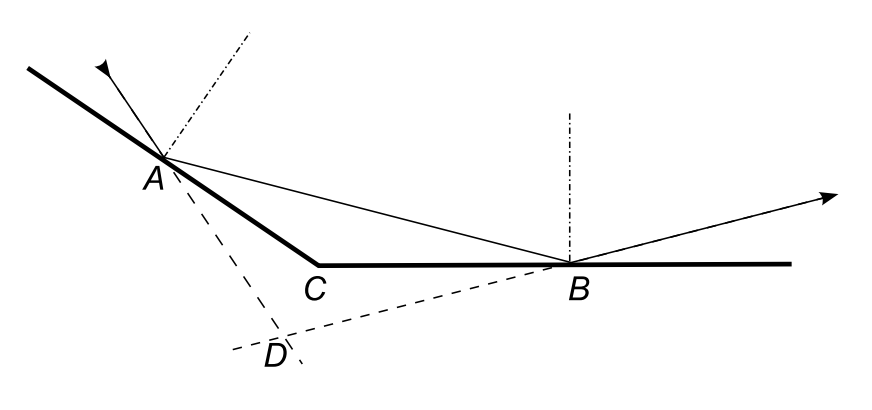
\includegraphics[width=0.5\linewidth]{2011-v2p-02-lah.PNG}
\end{center}
Vaatleme kolmnurka ABC. Tipu C juures on nurk $150^{\circ}$. Tipu A juures on peegeldumisseaduse järgi nurk $20^{\circ}$. Seega tipu B juures on nurk $10^{\circ}$. Vaatleme kolmnurka ABD. ∠CAD on tipunurgana $20^{\circ}$. Seega kolmnurga tipu A juures on nurk $40^{\circ}$. Sarnaselt on tipu B juures kolmnurga nurk $20^{\circ}$. Seega tipu D nurk on $120^{\circ}$ ja kõrvalekalde suurus on $180^{\circ} - 120^{\circ} = 60^{\circ}$ esialgsest suunast.
\fi
}
